\documentclass[letter]{article} 
\addtolength{\hoffset}{-2.25cm}
\addtolength{\textwidth}{4.5cm}
\addtolength{\voffset}{-3.25cm}
\addtolength{\textheight}{5cm}
\setlength{\parskip}{0pt}
\setlength{\parindent}{0in}

\usepackage[square,sort,comma,numbers]{natbib}
\usepackage{blindtext} % Package to generate dummy text
\usepackage{charter} % Use the Charter font
\usepackage[utf8]{inputenc} % Use UTF-8 encoding
\usepackage{microtype} % Slightly tweak font spacing for aesthetics
\usepackage{amsthm, amsmath, amssymb} % Mathematical typesetting
\usepackage{float} % Improved interface for floating objects
\usepackage{hyperref} % For hyperlinks in the PDF
\usepackage{graphicx, multicol} % Enhanced support for graphics
\usepackage{xcolor} % Driver-independent color extensions
\usepackage{pseudocode} % Environment for specifying algorithms in a natural way
\usepackage[ddmmyyyy]{datetime} % Uses YEAR-MONTH-DAY format for dates
\usepackage[spanish, activeacute, es-lcroman]{babel}

\usepackage{fancyhdr} % Headers and footers
\pagestyle{fancy} % All pages have headers and footers
\fancyhead{}\renewcommand{\headrulewidth}{0pt} % Blank out the default header
\fancyfoot[L]{} % Custom footer text
\fancyfoot[C]{} % Custom footer text
\fancyfoot[R]{\thepage} % Custom footer text
\newcommand{\note}[1]{\marginpar{\scriptsize \textcolor{red}{#1}}} % Enables comments in red on margin

\makeatletter
\renewcommand\subsection{\@startsection{subsection}{3}{\z@}%
                                     {-3.25ex\@plus -1ex \@minus -.2ex}%
                                     {-1.5ex \@plus -.2ex}% Formerly 1.5ex \@plus .2ex
                                     {\normalfont\normalsize\bfseries}}
\makeatother

\usepackage{listings}
\lstloadlanguages{[5.2]Mathematica}

\usepackage{enumerate}

\usepackage{subcaption}

\usepackage{dsfont}

\usepackage{wrapfig}

\usepackage{enumitem}

\usepackage{cancel}

\usepackage{booktabs}

%----------------------------------------------------------------------------------------


%-------------------------------
%	TITLE VARIABLES (identify your work!)
%-------------------------------

\newcommand{\firstname}{Nicolas Maldonado Baracaldo}
\newcommand{\firstid}{201423809}
\newcommand{\firstemail}{n.maldonado10@uniandes.edu.co}

\begin{document}

%-------------------------------
%	TITLE SECTION (do not modify unless you really need to)
%-------------------------------
\fancyhead[C]{}
\hrule \medskip
\begin{minipage}{0.295\textwidth} 
\raggedright
\footnotesize
\firstname \hfill\\ 
\firstid \hfill\\ 
\firstemail \hfill\\
\end{minipage}
\begin{minipage}{0.4\textwidth} 
\centering 
\large 
Estadística No Paramétrica y Remuestreo (MATE3526)\\
\normalsize
Adolfo J. Quiroz\\
Proyecto 1\\
\end{minipage}
\begin{minipage}{0.295\textwidth} 
\raggedleft
\today\hfill\\
\end{minipage}
\medskip\hrule 
\bigskip

\setlength{\parskip}{8pt}
\setlength{\parindent}{0.5in}

%-------------------------------
%	ASSIGNMENT CONTENT (add your responses)
%-------------------------------

En la teoría de estadística no paramétrica aparece una clase de estadísticos llamados \emph{$U$-estadísticos}, de particular importancia pues permiten realizar tests de hipótesis acerca de parámetros de distribuciones desconocidas y en estos casos pueden llegar a ser no-paramétricos libres de distribución. En particular para muestras independientes $X_1,\dots,X_m$ y $Y_1,\dots,Y_n$ de dos poblaciones con distribuciones en alguna familia dada, a un parámetro $\gamma$ se le llama \emph{estimable de grado} $(r,s)$ si $r$ y $s$ son los tamaños de muestra más pequeños para los cuales existe una función $h$ tal que

\begin{align*}
    \operatorname{E}[h(X_1,\dots,X_r,Y_1,\dots,Y_s)] = \gamma.
\end{align*}

En dado caso, a la función $h$ (la cual puede asumirse simétrica en los $X_i$s y simétrica en los $Y_j$s, pues incluso si no lo es se puede simetrizar) se le llama el \emph{kernel} del $U$-estadístico y éste último se define como

\begin{align*}
    U(X_1,\dots,X_m,Y_1,\dots,Y_n) = \frac{1}{{m \choose r}{n \choose s}}\sum_{\alpha \in A}\sum_{\beta \in B} h(X_{\alpha_1},\dots,X_{\alpha_r},Y_{\beta_1},\dots,Y_{\beta_s}).
\end{align*}

Más aún, el Teorema para $U$-Estadísticos de Dos Muestras nos garantiza que si $\operatorname{E}[h^2(X_1,\dots,X_r,Y_1,\dots,Y_s)]$ es finita, entonces $\sqrt{N}\left[U(X_1,\dots,X_m,Y_1,\dots,Y_n) - \gamma\right]$ tiene una distribución límite normal con media 0 y varianza $[r^2\zeta_{1,0}/\lambda] + [s^2\zeta_{0,1}/(1-\lambda)]$.\cite[Capítulo 3]{Randles1991IntroductionStatistic}

A continuación se quiere evaluar, para muestras provenientes de distribuciones $F(x/\eta_1)$ y $F(x/\eta_2)$, el $U$-estadístico de diferencia de escala con kernel

\begin{align*}
    h(x_1,x_2,y_1,y_2) = \Psi(|y_1 - y_2| - |x_1 - x_2|)
\end{align*}

para $H_0$ la hipótesis $\eta_1 = \eta_2$ y $H_a$ la hipótesis $\eta_1 < \eta_2$ usando el método de Monte Carlo, pues la estimación usando directamente $U$-estadísticos resulta computacionalmente demasiado costosa para grandes muestras.

(Todo lo que sigue se realizo usando \texttt{Mathematica}. El archivo \texttt{.nb} se adjunta al presente informe.)

\begin{enumerate}
\setcounter{enumi}{0}

\item Para empezar se definieron las funciones $\Psi$ y $h$ que se usarán para todos los cálculos. Se definieron los tamaños de las muestras, $m = 5000, n = 2000$, y se tomaron las muestras usando la función \texttt{RandomVariate} y proporcionando la distribución apropiada (\texttt{GammaDistribution}) con sus parámetros.

\item A continuación se definió el número de iteraciones a usar para Monte Carlo, $L = 2000$, y se procedió a usar el método para estimar $\zeta_{1,0}$ y $\zeta_{0,1}$. Se separó la muestra $X$ en dos para esta parte, luego se tomaron subconjuntos de tamaño 3 y 4 (resp. 4 y 3) de cada mitad usando la función \texttt{RandomSample} y con ellos se calculó

\begin{align*}
    \operatorname{est}\zeta_{1,0} = h(x_1,x_2,y_1,y_2)h(x_1,x_3,y_3,y_4) - \gamma^2
\end{align*}

(resp. $\operatorname{est}\zeta_{0,1}$), luego se tomó el promedio de éstos como valor para $\zeta_{1,0}$ (resp. $\zeta_{0,1}$). Finalmente, usando los estimados anteriores, así como $\lambda = m/N$, se estimó $\Tilde{\sigma}_U$.

\item Usando el mismo número de iteraciones que antes, se estimó mediante el método de Monte Carlo el $U$-estadístico con kernel $h$. Para esta parte se tomaron subconjuntos de $X$ y de $Y$ por separado, ambos de tamaño 2, de nuevo con la función \texttt{RandomSample} y se calculó $h(x_1,x_2,y_1,y_2)$, el cual luego se promedió para dar un estimado del $U$-estadístico. Por último se usó éste y el estimado anterior para calcular $\Tilde{U} = \sqrt{N}(U - \gamma)/\Tilde{\sigma}_U$, el cual según el teorema ya citado debería tener una distribución normal estándar.

\item En este punto se quería repetir todo el proceso 500 veces para evaluar la normalidad de $\Tilde{U}$, por lo que resultó conveniente definir una nueva función \texttt{MC} que realizara todo esto dados los parámetros $m,n,sX,sY,L$, donde $m,n,L$ tienen las mismas definiciones que en los procedimientos anteriores y $sX,sY$ se refieren a los parámetros de escala a ingresar a \texttt{GammaDistribution} al momento de tomar las muestras $X$ y $Y$, respectivamente (esto con el fin de que la misma función nos sirva para evaluar tanto la hipótesis nula como la alternativa). Teniendo esta función definida, se generaron los 500 valores usando la función \texttt{Table} con el llamado a la función $MC$ con $m = 5000, n = 2000, sX = 2, sY = 2, L = 2000$. Se evaluó en este punto la normalidad mediante tres métodos,

\begin{enumerate}[label=(\roman*)]

\item Se generó un q-q plot usando la función \texttt{QuantilePlot} (figura \ref{fig:H0}).

\begin{figure}[h!]
    \centering
    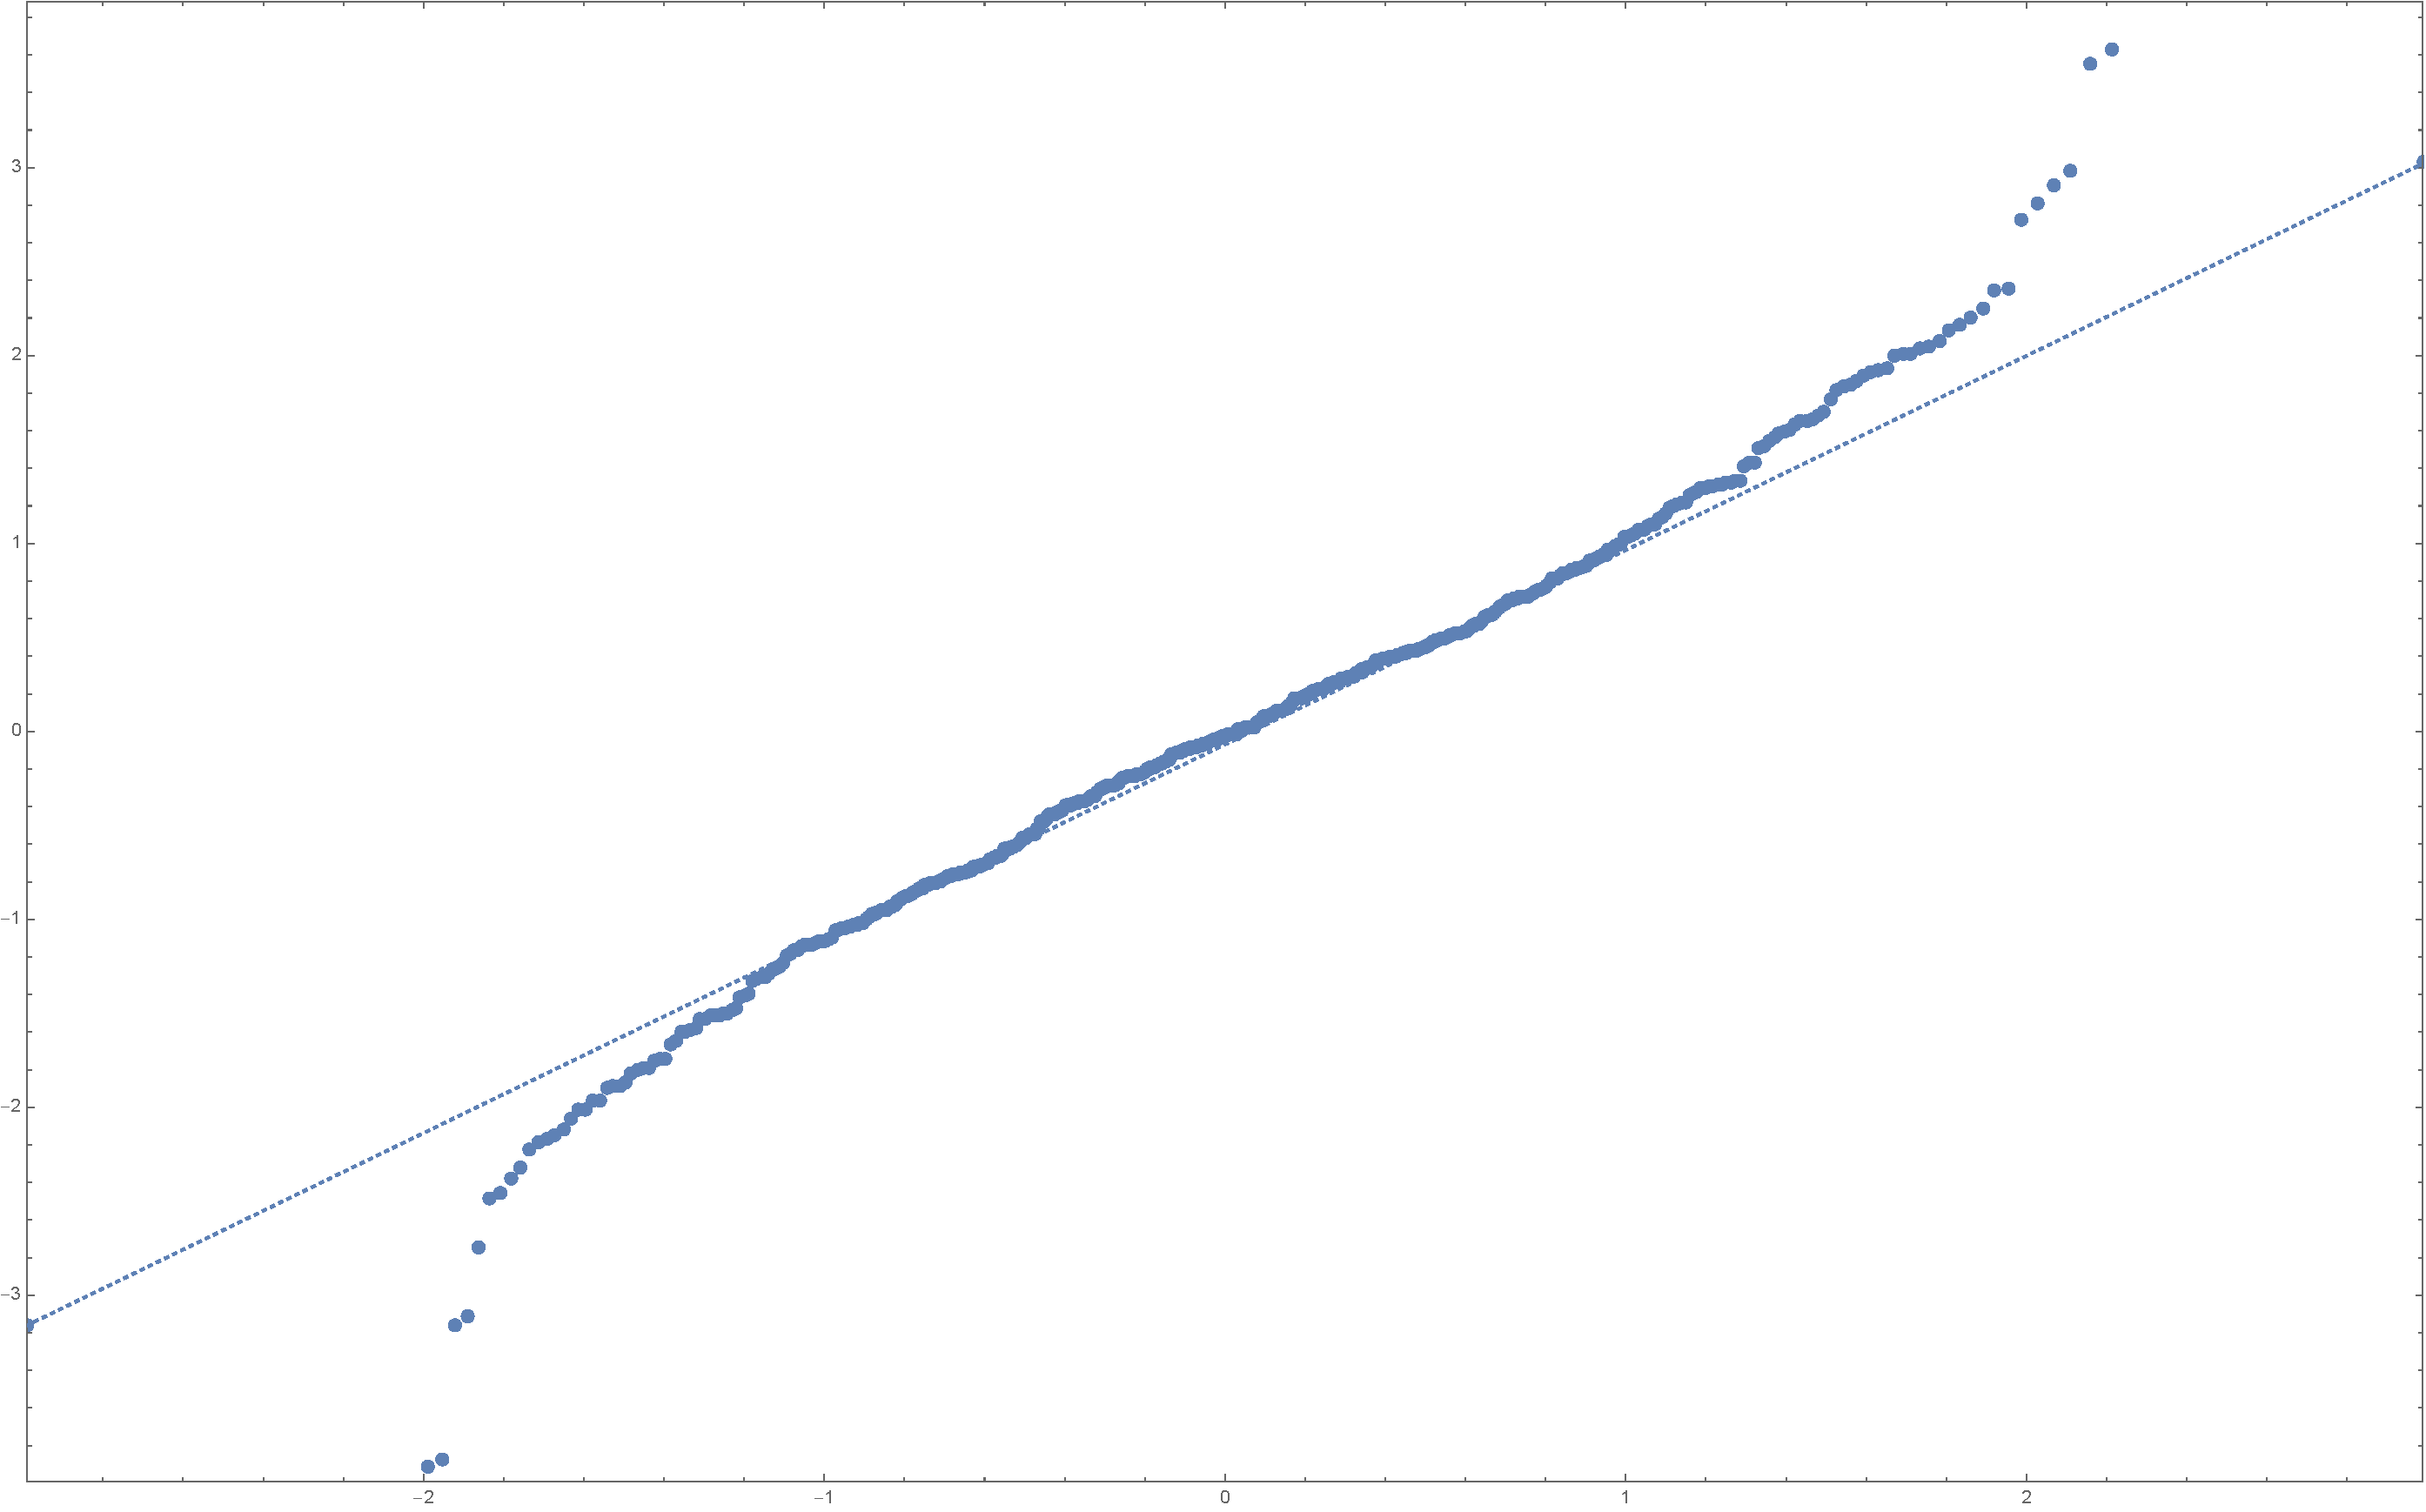
\includegraphics[width=0.6\textwidth]{q-q_H0.pdf}
    \caption{q-q plot obtenido para $H_0$.}
    \label{fig:H0}
\end{figure}

\item Se realizó el test de Cramér-von Mises usando la función \texttt{CramerVonMisesTest}, el cual arrojó el resultado ``\emph{The null hypothesis that the data is distributed according to the NormalDistribution[0, 1] is not rejected at the 5 percent level based on the Cramér-von Mises test.}''.

El test de Cramér-von Mises básicamente usa la suma de diferencias cuadradas entre las FDAs esperada y observada como estadístico de prueba.

Se realizó también el test de Kolmogorov-Smirnov usando la función \texttt{KolmogorovSmirnovTest}, el cual arrojó el resultado ``\emph{The null hypothesis that the data is distributed according to the NormalDistribution[0, 1] is not rejected at the 5 percent level based on the Kolmogorov-Smirnov test.}''.

El test de Kolmogorov-Smirnov básicamente usa el supremo de los valores absolutos de las diferencias entre las FDAs esperada y observada como estadístico de prueba.

\item Se contó el porcentaje de veces que $\Tilde{U}$ sobrepasó el cuantil 95\% de la normal estándar. Para la corrida en que se realizó el conteo se obtuvo aquí que un $7.8\%$ de los datos excedían el cuantil.

\end{enumerate}

\item Con base en las diversas evaluaciones de normalidad realizadas, es razonable concluir que bajo $H_0$ en efecto se tiene que $\Tilde{U}$ calculado mediante Monte Carlo seguirá una distribución normal estándar, tal y como se quería.

\item A continuación se quería seguir básicamente el mismo proceso para la hipótesis alternativa. Se aprovechó acá que ya se había definido la función \texttt{MC}, y se generaron los 500 valores usando la función \texttt{Table} con el llamado a la función $MC$ con $m = 5000, n = 2000, sX = 2, sY = 3, L = 2000$. Se evaluó en este punto la normalidad mediante los mismos tres métodos,

\newpage

\begin{enumerate}[label=(\roman*)]

\item Se generó un q-q plot usando la función \texttt{QuantilePlot} (figura \ref{fig:Ha}).

\begin{figure}[h!]
    \centering
    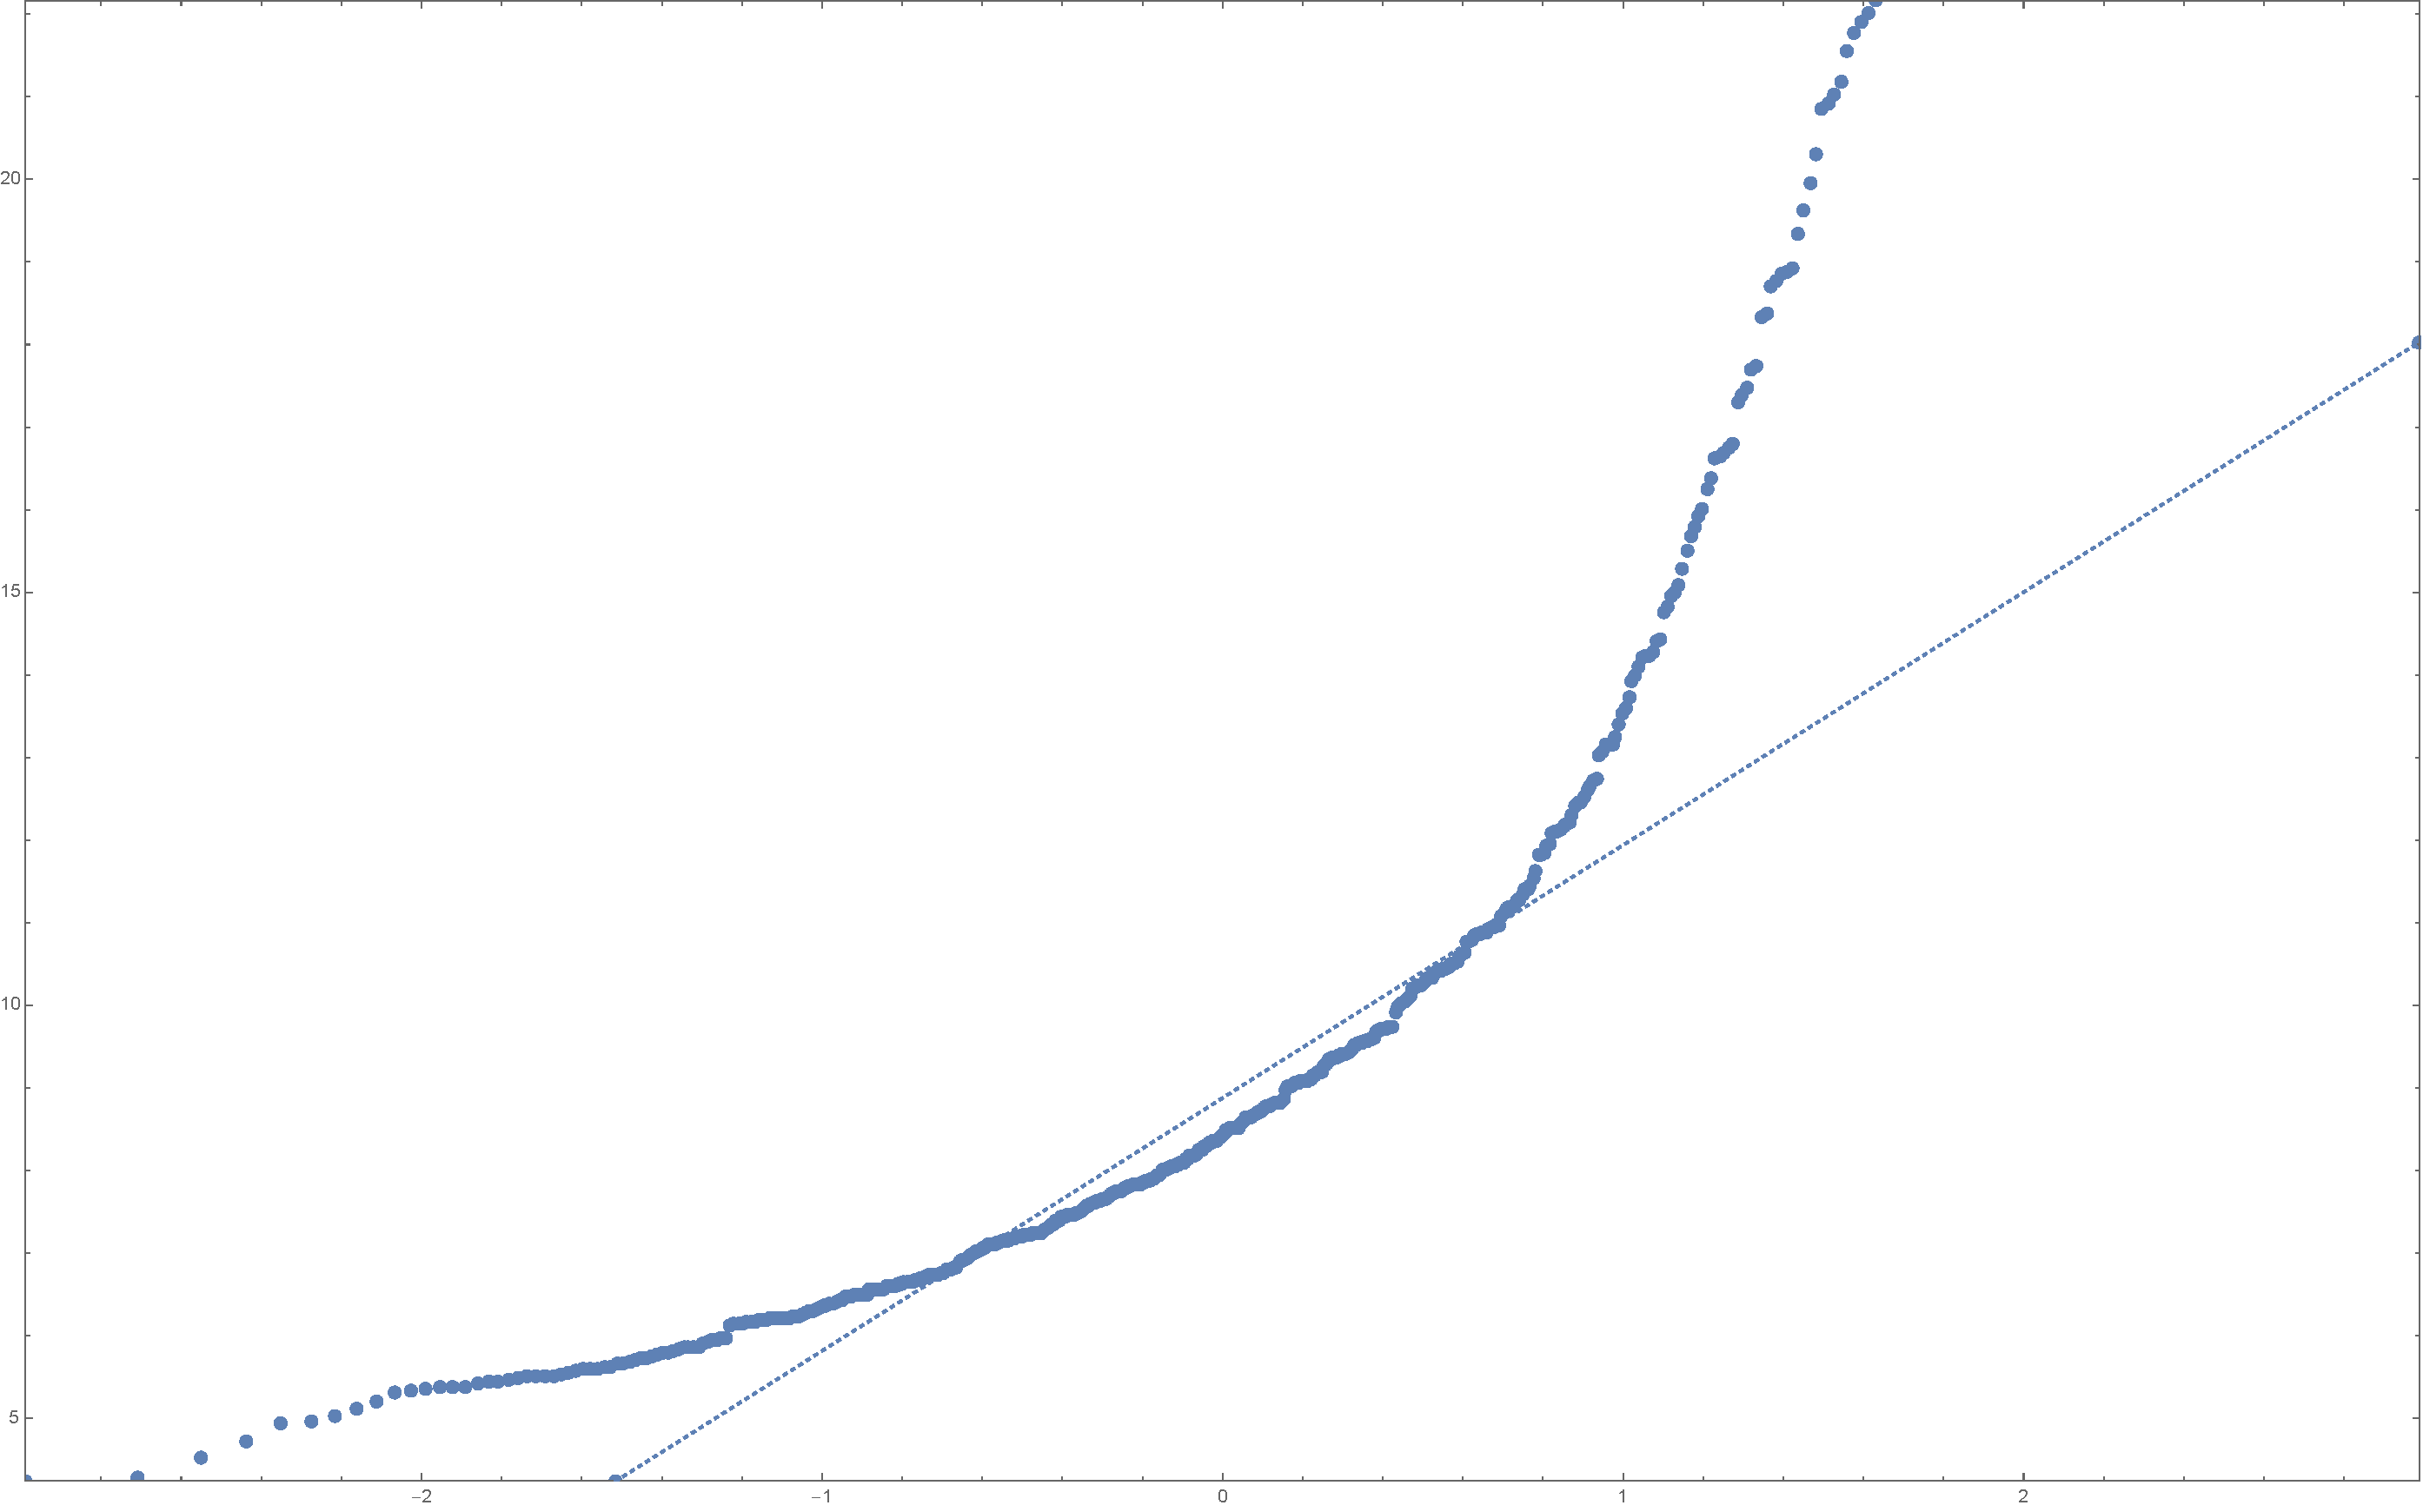
\includegraphics[width=0.6\textwidth]{q-q_Ha.pdf}
    \caption{q-q plot obtenido para $H_a$.}
    \label{fig:Ha}
\end{figure}

\item Se realizó el test de Cramér-von Mises usando la función \texttt{CramerVonMisesTest}, el cual arrojó el resultado ``\emph{The null hypothesis that the data is distributed according to the NormalDistribution[0, 1] is rejected at the 5 percent level based on the Cramér-von Mises test.}''.

Se realizó también el test de Kolmogorov-Smirnov usando la función \texttt{KolmogorovSmirnovTest}, el cual arrojó el resultado ``\emph{The null hypothesis that the data is distributed according to the NormalDistribution[0, 1] is rejected at the 5 percent level based on the Kolmogorov-Smirnov test.}''.

\item Se contó el porcentaje de veces que $\Tilde{U}$ sobrepasó el cuantil 95\% de la normal estándar. Para la corrida en que se realizó el conteo se obtuvo aquí que un $100\%$ de los datos excedían el cuantil.

\end{enumerate}

\item Con base en las diversas evaluaciones de normalidad realizadas, es razonable concluir que bajo $H_a$ no se tiene que $\Tilde{U}$ calculado mediante Monte Carlo seguirá una distribución normal estándar, luego garantizamos que dadas muestras desconocidas, se podrá usar como test de hipótesis el estadístico así calculado, junto con algún tipo de criterio de normalidad.

\end{enumerate}

Como ya se mencionó, el hecho de que hayamos podido usar el método de Monte Carlo para estimar $\Tilde{U}$ en los dos casos, y que se tenga normalidad en su distribución únicamente cuando se cumple $H_0$, nos da entonces que este es un método sensato y razonable para evaluar las hipótesis $H_0$ y $H_a$ relacionadas con el parámetro de escala de las dos muestras incluso en el caso en que no conozcamos la distribución de la que provienen. En adelante dadas dos muestras independientes se puede usar el método aquí presentado para estimar $\Tilde{U}$ y luego un sencillo test de normalidad nos permitirá evaluar nuestras hipótesis.

Más allá de lo aquí realizado, esto también nos indica que incluso para muestras de tamaño muy grande los $U$-estadísticos no se vuelven inútiles. Si bien su cálculo directo ya no va a ser factible en estos casos, hemos visto que el uso del método de Monte Carlo no los hace menos poderosos. Claro está que aquí solo se evaluó para un $U$-estadístico particular, sin embargo los resultados son prometedores y fácilmente se podrían realizar evaluaciones similares para cualquier estadístico previo a su uso si igualmente se quiere estar seguro.

\bibliographystyle{unsrt}
\bibliography{references.bib}

\end{document}